

\newcommand{\FigTx}{
\begin{figure*}[ht]
    \centering
    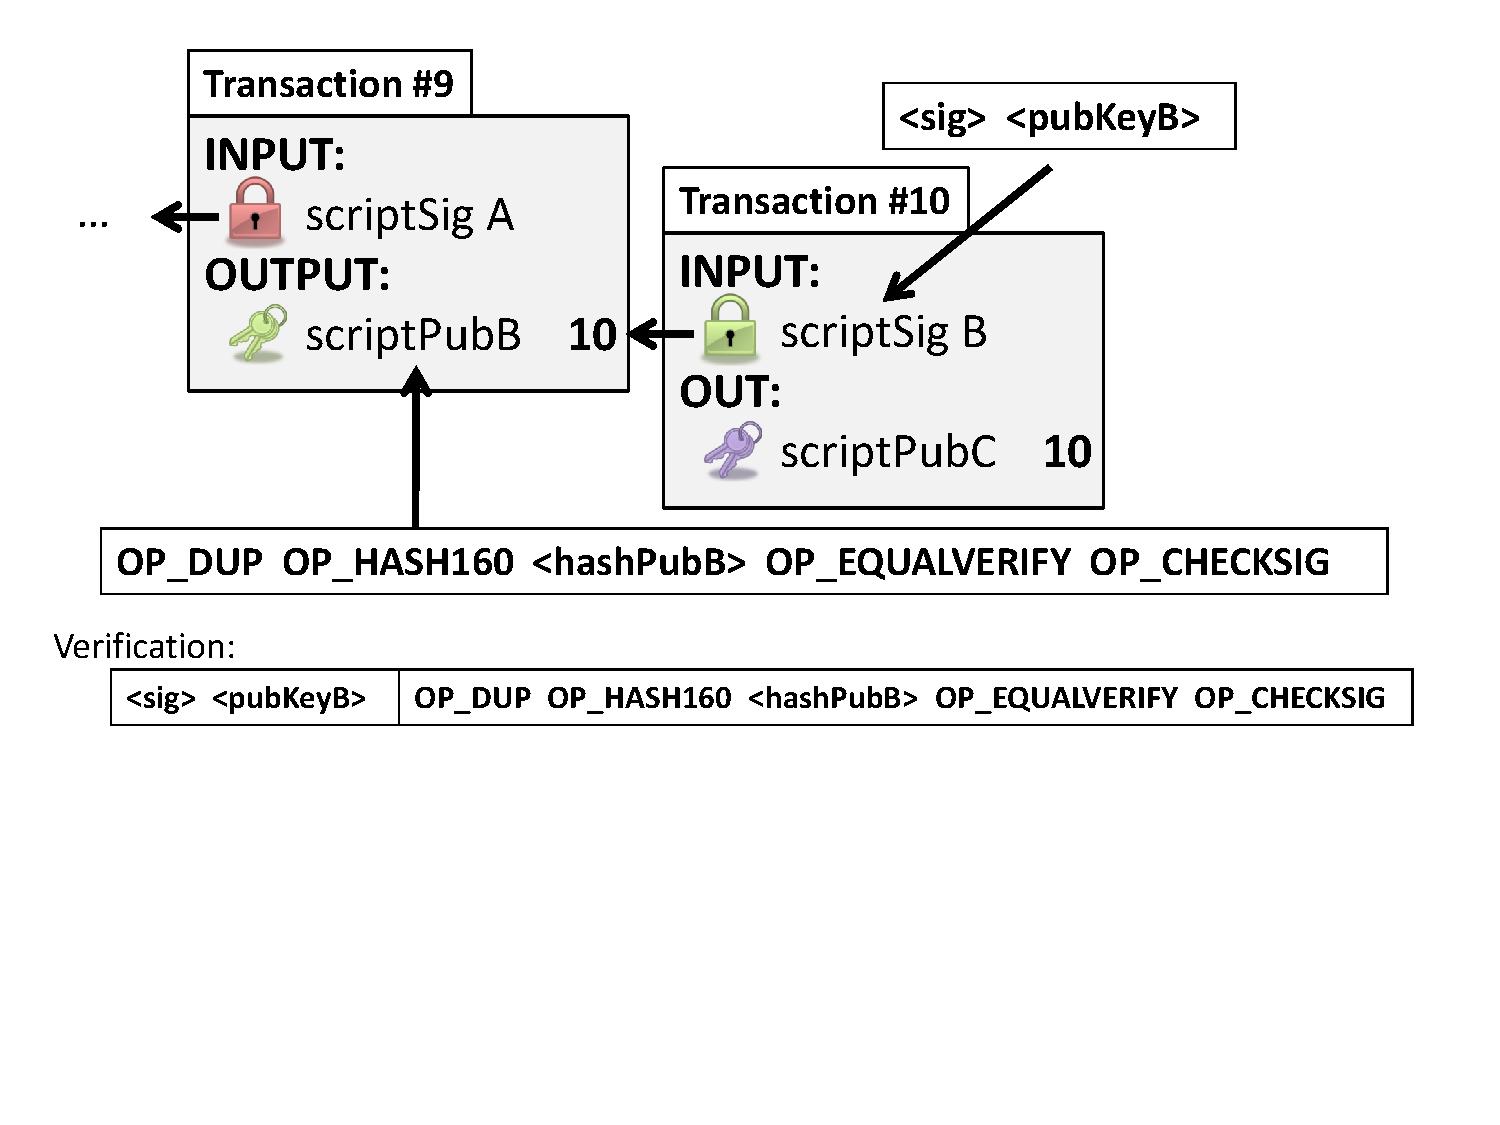
\includegraphics[width=0.9\textwidth,trim={0 6.5cm 1cm 0},clip]{btc-transaction.pdf}
    \caption{\textbf{Standard Bitcoin transaction script}\,--\, %
            Transaction \#10 spends \#9 by providing a
            valid input script that when prepended to Transaction \#9's output script,
            executes to produce a valid output. The output script stores a hash of a
            public key (verified using the OP\_DUP OP\_HASH160 and OP\_EQUALVERIFY opcodes),
            and requires a valid signature over the spending transaction (verified via
            OP\_CHECKSIG).}
    \label{fig:bitcoin-tx}
\end{figure*}
}

\newcommand{\FigTLS}{
\begin{figure*}[ht]
    \centering
    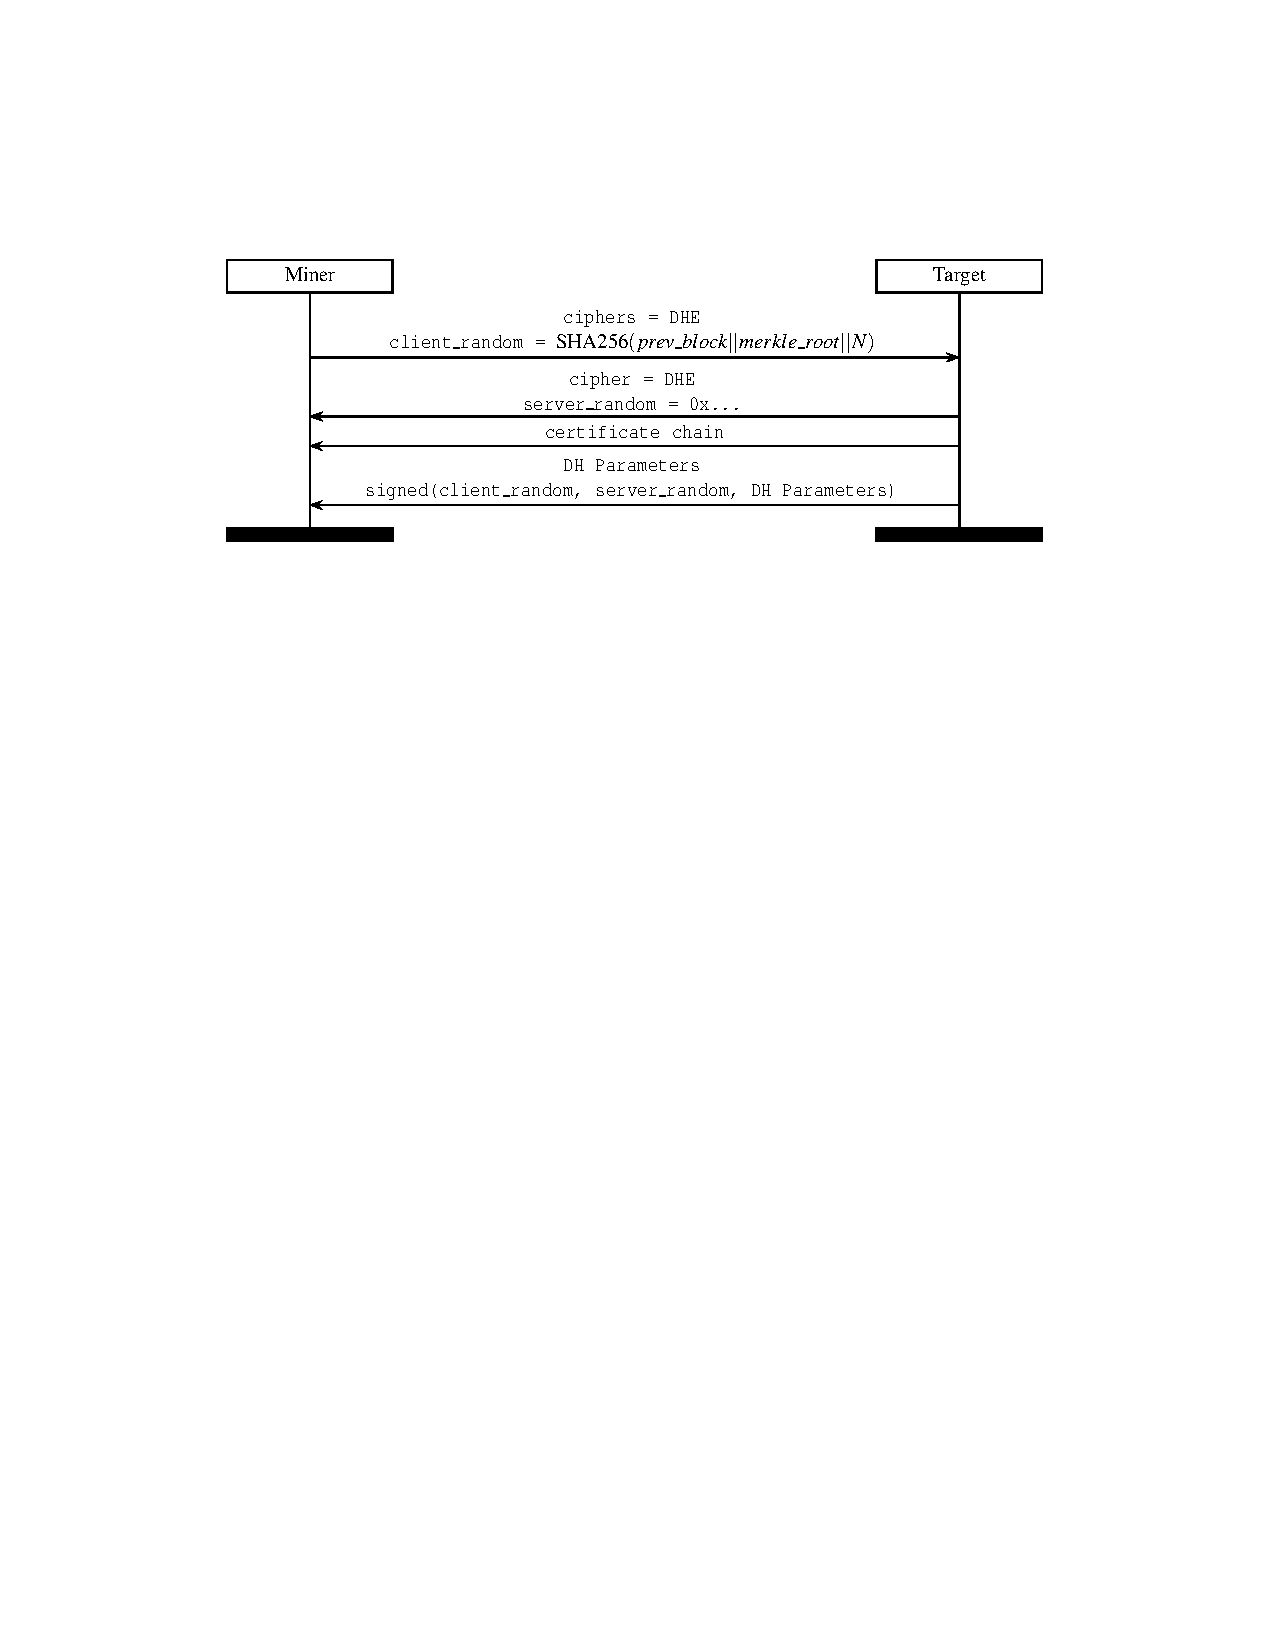
\includegraphics[width=0.9\textwidth,clip]{figures/tls.pdf}
    \caption{\textbf{Miner--Target Interaction}\,--\, %
	A single round-trip is required for each attempt to solve the proof-of-work. The client
	computes the \texttt{client\_random} to commit to a given previous block and set of 
	transactions, and only provides the server the option to use Diffie-Hellman Ephemeral
	cipher-suites. The server then calculates a signature dependent on the 
	\texttt{client\_random} and verifiable by the certificate the server provides.
}
    \label{fig:tls-connection}
\end{figure*}
}

\newcommand{\FigOverview}{
\begin{figure*}[ht]
    \centering
    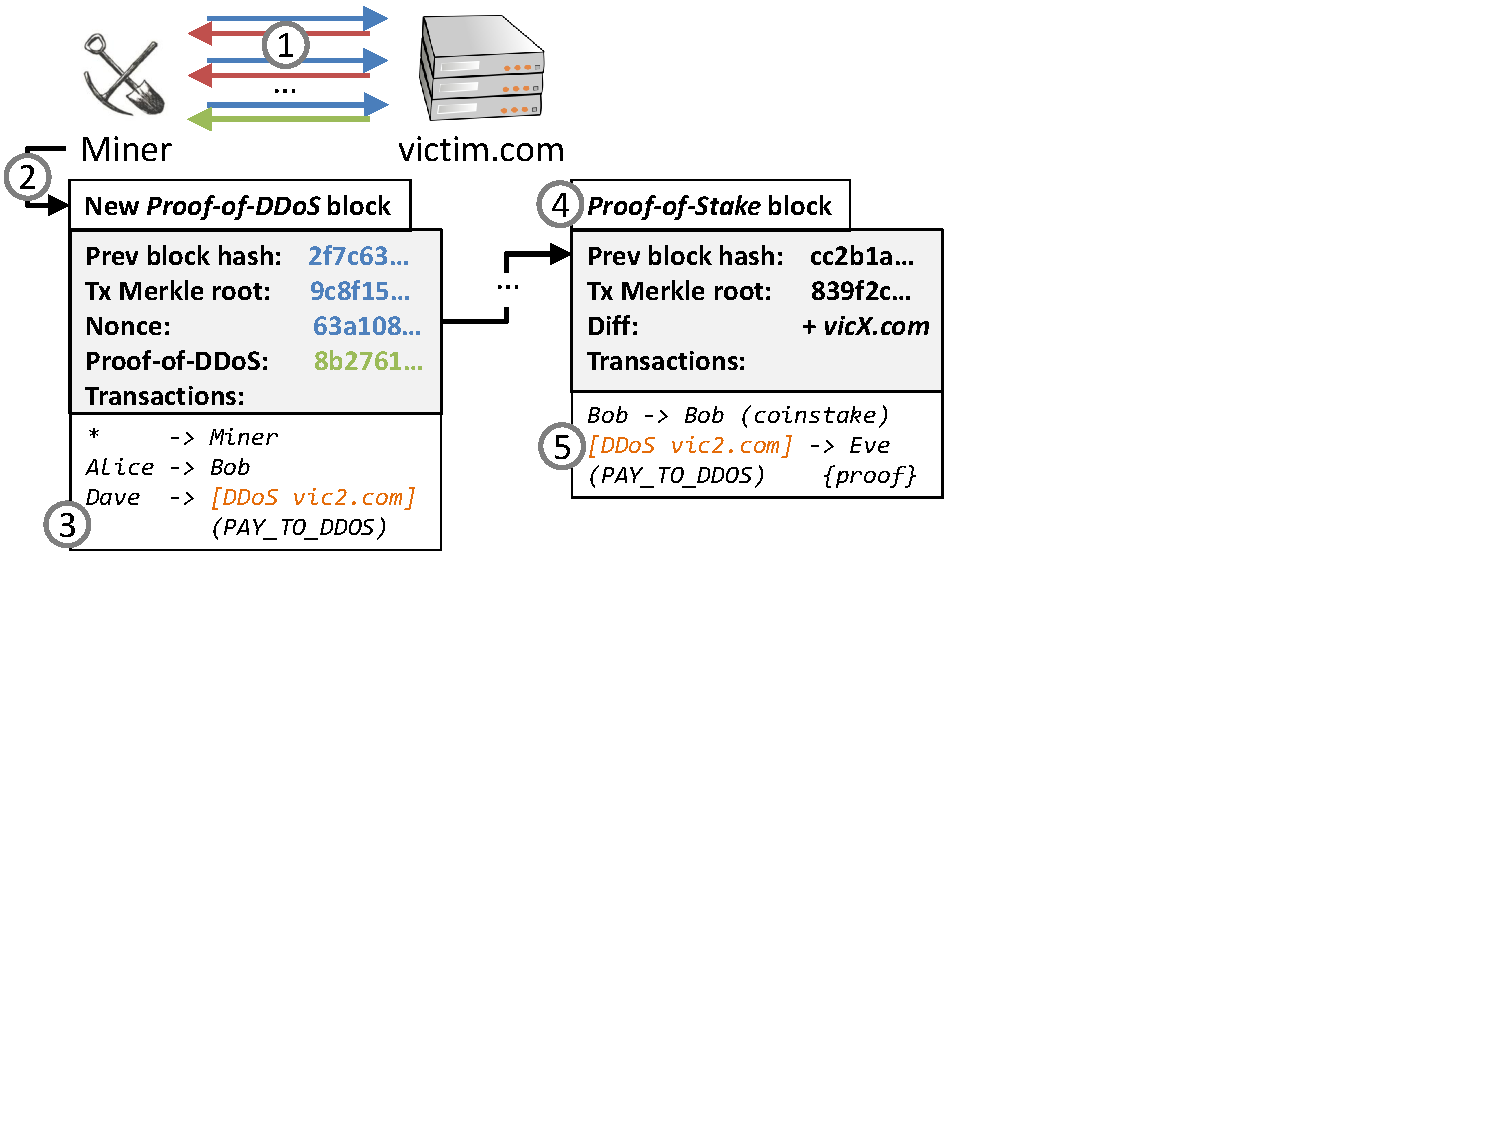
\includegraphics[width=0.9\textwidth,trim={0 9.5cm 9.2cm 0},clip]{ddoscoin-overview.pdf}
    \caption{\textbf{DDoSCoin Design}\,--\, %
    DDoSCoin miners make repeated connections to a victim server running TLSv1.2
\numcircledmod{1}. In each handshake, the miner commits to the previous block, a transaction
merkle root, and a secret nonce. Eventually the victim server will respond with
a signed message that meets the current proof-of-DDoS target difficulty, and the miner can
create a new block \numcircledmod{2} that includes this proof. Victim targets can be selected
in two ways: First, participants can pay into one-time bounties for specific
victims \numcircledmod{3}, which can be redeemed by anyone in a special PAY\_TO\_DDOS
transaction \numcircledmod{5} if they can provide a similar proof-of-DDoS against that victim. Second, the list of
valid victims that blocks can be mined for can be updated by proof-of-stake
blocks \numcircledmod{4}.}
    \label{fig:ddoscoin-overview}
\end{figure*}
}

\newcommand{\FigEval}{
\begin{figure}[t]
    \centering
    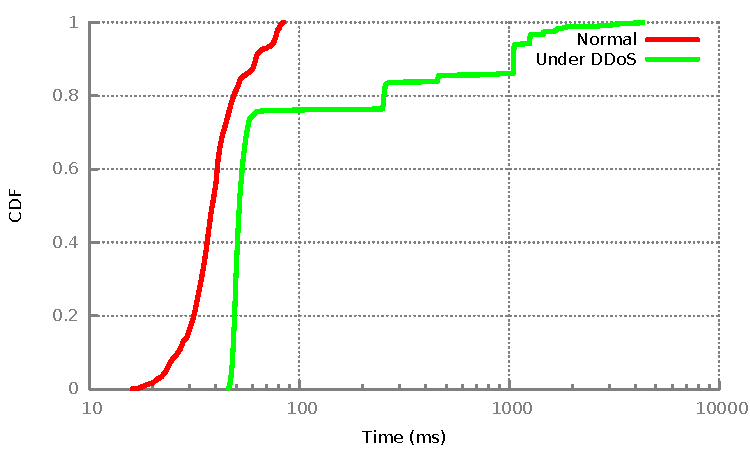
\includegraphics[width=0.9\linewidth]{../data/times.pdf}
    \caption{\textbf{DDoSCoin effect}\,--\, %
    We set up a quad-core nginx HTTPS server on a local network, and used Apache
benchmark (ab) to measure page load times under normal conditions (no DDoSCoin
miner running) and with a single DDoSCoin instance. DDoSCoin increases the
average page-load time 6-fold from 43ms to over 291ms.}
    \label{fig:eval}
\end{figure}
}
